\documentclass[../main.tex]{subfiles}
\begin{document}

    Odpowiedź na syndrom \textbf{LOOP} - \textbf{L}ate, \textbf{O}ver budget, \textbf{O}vertime, \textbf{P}oor quality.

    Minusy standaryzacji:
    \begin{itemize}
        \item Ważniejszy proces niż samo oprogramowanie,
        \item Spora cześć procesu jest fikcyjna, tworzenie dużej ilości dokumentacji,
        \item Dyscyplina zabija inicjatywę.
    \end{itemize}

    \subsection{CMM - Capability Maturity Model}
    \textbf{Ocenia proces wytwórczy} służacy do produkcji oprogramowania w skali pięciostopniowej - od \textbf{chaotycznego} (nic nie jest
    sterowane ani kontrolowane), aż do \textbf{ścisłego}, zdyscyplinowanego procesu uwzględniającego wszystkie potrzebne aspekty.

    Model CMM obejmuje \textbf{pięć aspektów}:
    \begin{itemize}
        \item Poziomy dojrzałości
        \item Kluczowe obszary procesowe
        \item Cele
        \item Atrybuty procesu
        \item Kluczowe praktyki
    \end{itemize}

    \subsubsection{Poziomy dojrzałości}
    \begin{table}[H]
        \begin{center}
            \begin{tabular}{ p{8cm} p{8cm} }
                \textbf{Poziom 1 - Wstępny}
                &
                \begin{itemize}
                    \item Działanie tymczasowe, doraźne.
                    \item Organizacja bez stabilnej technologii wytwarzania i utrzymywania produktów.
                    \item Zakres projektów zupełnie nieprzewidywalny.
                \end{itemize}
                \\

                \textbf{Poziom 2 - Powtarzalny}
                &
                \begin{itemize}
                    \item Dokumentowane standardy dokumentacji, szkoleń, utrzymywania.
                    \item W miarę ustabilizowane środowisko pracy i procedury zarządzania.
                \end{itemize}
                \\

                \textbf{Poziom 3 - Zdefiniowany}
                &
                \begin{itemize}
                    \item Spójny zbiór definicji i standardów na poziomie
                    organizacji realizującej projekt.
                    \item Wyodrębnienie w zespole specjalistów od realizacji
                    poszczególnych zadań, a organizacja dąży do wyposażenia ich
                    w niezbędną wiedzę i umiejętności.
                    \item Organizacja zaczyna na podstawie własnych doświadczeń
                    modyfikować sposób prowadzenia projektów, tak aby
                    maksymalnie odpowiadał jej specyfice.
                \end{itemize}
                \\

                \textbf{Poziom 4 - Zarządzany}
                &
                \begin{itemize}
                    \item W jakimś zdefiniowanym obszarze wyniki podejmowanych działań
                    przenoszą określone rezultaty, które można zmierzyć za
                    pomocą wcześniej zdefiniowanych metryk.
                    \item Zadania, których wykonanie nie generuje dużej liczby
                    błędów mogą być kontrolowane z mniejszą
                    częstotliwością, zaś obszary zdefiniowane jako
                    potencjalnie niebezpieczne np. w związku ze zmianą
                    technologii, mogą podlegać ściślejszej kontroli.
                \end{itemize}
                \\

                \textbf{Poziom 5 - Optymalizujący}
                &
                \begin{itemize}
                    \item Proces jest już tak dobrze zorganizowany i zarządzany, że
                    nie pozostaje nic innego, jak tylko dalsze podnoszenie
                    stawianych przed procesem wymagań.
                    \item Celem stawianym na tym poziomie jest optymalizacja i
                    dalsze ulepszanie procesu, zwiększanie jego
                    efektywności oraz wydajności.
                \end{itemize}
                \\
            \end{tabular}
        \end{center}
    \end{table}


    \subsection{ISO 9000}
    Wymaga \textbf{udokumentowania wszystkich procedur} związanych z wytwarzaniem oprogramowania.

    \begin{figure}[H]
        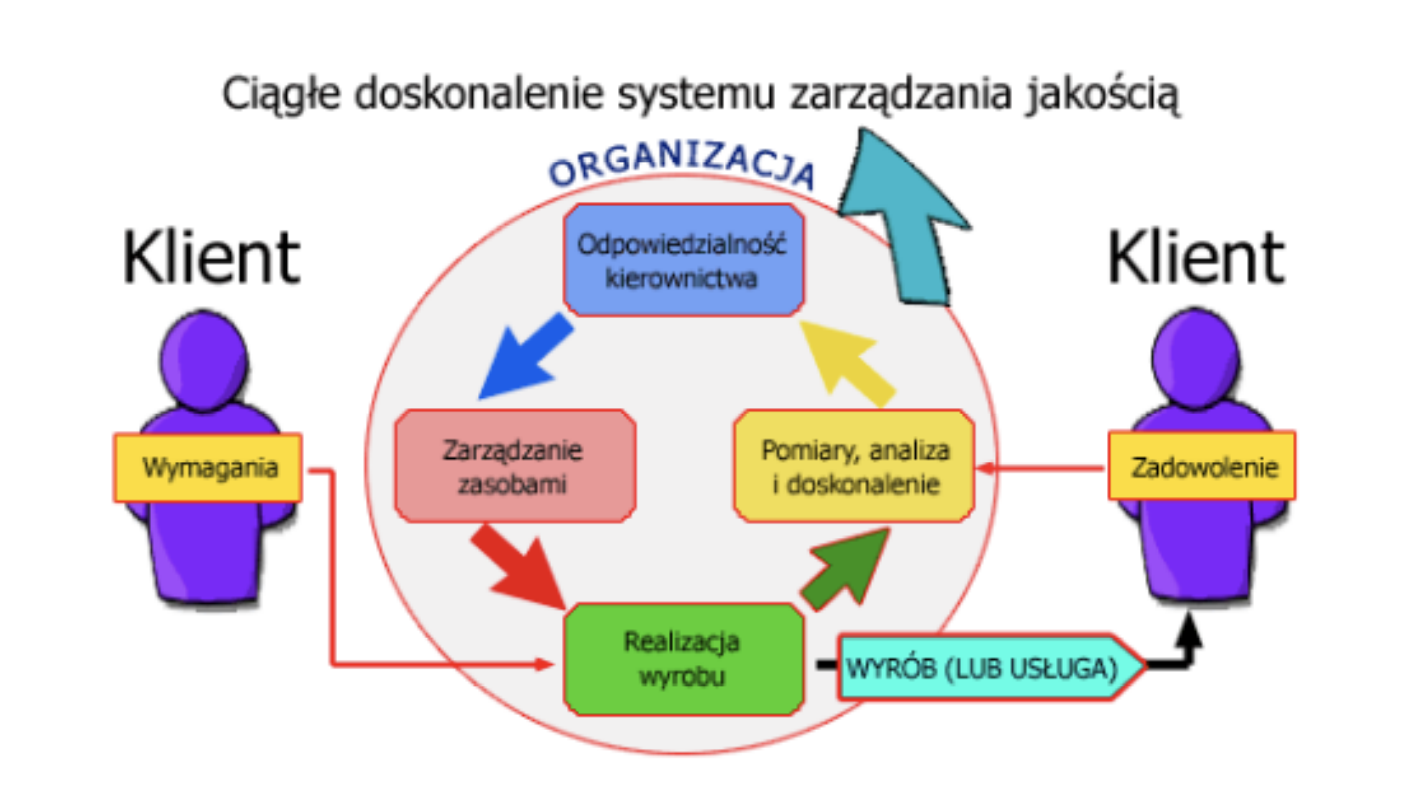
\includegraphics[width=\linewidth]{model_ISO.png}
    \end{figure}

    \begin{table}[H]
        \begin{center}
            \begin{tabular}{ p{8cm} p{8cm} }
                \textbf{Odpowiedzialność kierownictwa}
                &
                Kierownictwo:
                \begin{itemize}
                    \item odpowiada za właściwe funkcjonowanie organizacji,
                    \item ustala misję i politykę organizacji, określa cele,
                    \item opracowuje plan
                    działań do realizacji celów i przyznaje odpowiednie zasoby.
                \end{itemize}
                \\

                \textbf{Zarządzanie zasobami}
                &
                \begin{itemize}
                    \item Zespół procesów związanych z zasobami - ludzkimi, infrastrukturą, środowiskiem pracy.
                \end{itemize}
                \\

                \textbf{Realizacja wyrobu}
                &
                \begin{itemize}
                    \item Zespół procesów bezpośrednio związany z
                    realizacją wyrobu lub usługi.
                    \item Wejściem są wymagania klienta, a wyjściem jest
                    dostarczony wyrób lub usługa.
                \end{itemize}
                \\

                \textbf{Pomiary, analiza i doskonalenie}
                &
                \begin{itemize}
                    \item Procesy w organizacji i zadowolenie klienta
                    wymagają systematycznego monitoringu, analizy i
                    podejmowania działań doskonalących, aby wiedzieć
                    jak postrzega nas klient (zadowolenie) oraz jak
                    funkcjonują procesy w organizacji (zielona strzałka).
                \end{itemize}
                \\

                \textbf{Ciągłe doskonalenie} systemu zarządzania jakością
                &
                \begin{itemize}
                    \item Ciągłe zwiększanie skuteczności i efektywności w realizacji polityki,
                    strategii i celów organizacji.
                \end{itemize}
                \\
            \end{tabular}
        \end{center}
    \end{table}



\end{document}